\documentclass[12pt]{article}

\usepackage{amsmath}
\usepackage{amssymb}
\usepackage{amsthm}
\usepackage[pdftex]{graphicx}
\usepackage{setspace}
\usepackage{caption}
\usepackage{subcaption}
\usepackage{float}
\usepackage[margin=1in]{geometry}
\usepackage{listings}
\usepackage{textcomp}
\usepackage{multicol}
\usepackage[toc,page]{appendix}
\usepackage{listings}
\usepackage{fancyvrb}
\usepackage{hyperref}
\usepackage{lstbayes}

\usepackage[usenames,dvipsnames]{color}

%\usepackage{algorithm}
%\usepackage{algpseudocode}
\usepackage[ruled,vlined,linesnumbered]{algorithm2e}
\newcommand\mycommfont[1]{\footnotesize\ttfamily\textcolor{Gray}{#1}}
\SetCommentSty{mycommfont}
%\floatname{algorithm}{Procedure}
%\renewcommand{\algorithmicrequire}{\textbf{Input:}}
%\renewcommand{\algorithmicensure}{\textbf{Output:}}
%\makeatletter
%\def\therule{%
%  \makebox[\algorithmicindent][l]{%
%    \hspace*{.5em}\vrule height .75\baselineskip depth .25\baselineskip}}%

\usepackage{inconsolata}

\usepackage[parfill]{parskip}
\setlength{\parindent}{0pt}
\setlength{\parskip}{\baselineskip}

\newcommand{\et}{e^{i\theta}}
\newcommand{\oo}{\mathcal{O}}
\newcommand{\skipline}{\bigskip\bigskip\bigskip}

\lstdefinestyle{Rsty} { 
    language=R,                         % the language of the code
    basicstyle=\footnotesize\ttfamily,  % the size of the fonts that are used for the code
    numbers=left,                       % where to put the line-numbers
    numberstyle=\footnotesize\color{Blue},      % the style that is used for the line-numbers
    stepnumber=1,                       % the step between two line-numbers. If it is 1, each line
                                        % will be numbered
    numbersep=5pt,                      % how far the line-numbers are from the code
    backgroundcolor=\color{white},      % choose the background color. You must add \usepackage{color}
    showspaces=false,                   % show spaces adding particular underscores
    showstringspaces=false,             % underline spaces within strings
    showtabs=false,                     % show tabs within strings adding particular underscores
    %frame=single,                       % adds a frame around the code
    rulecolor=\color{black},            % if not set, the frame-color may be changed on line-breaks within not-black text (e.g. commens (green here))
    tabsize=2,                          % sets default tabsize to 2 spaces
    captionpos=b,                       % sets the caption-position to bottom
    breaklines=true,                    % sets automatic line breaking
    breakatwhitespace=false,            % sets if automatic breaks should only happen at whitespace
    keywordstyle=\color{RoyalBlue},     % keyword style
    commentstyle=\color{YellowGreen},   % comment style
    stringstyle=\color{ForestGreen},    % string literal style
    literate={<-}{{$\gets$}}1,           % prettier assignment arrows
    xleftmargin=4.0ex,
    deletekeywords={I,density,rect,_,palette,data,scale,panel,R,frame,labels,options}
}

\lstnewenvironment{R}
{\lstset{style=Rsty}}
{}

\lstdefinestyle{Stansty} { 
    language=Stan,                         % the language of the code
    basicstyle=\footnotesize\ttfamily,  % the size of the fonts that are used for the code
    numbers=left,                       % where to put the line-numbers
    numberstyle=\footnotesize\color{Blue},      % the style that is used for the line-numbers
    stepnumber=1,                       % the step between two line-numbers. If it is 1, each line
                                        % will be numbered
    numbersep=5pt,                      % how far the line-numbers are from the code
    backgroundcolor=\color{white},      % choose the background color. You must add \usepackage{color}
    showspaces=false,                   % show spaces adding particular underscores
    showstringspaces=false,             % underline spaces within strings
    showtabs=false,                     % show tabs within strings adding particular underscores
    %frame=single,                       % adds a frame around the code
    rulecolor=\color{black},            % if not set, the frame-color may be changed on line-breaks within not-black text (e.g. commens (green here))
    tabsize=2,                          % sets default tabsize to 2 spaces
    captionpos=b,                       % sets the caption-position to bottom
    breaklines=true,                    % sets automatic line breaking
    breakatwhitespace=false,            % sets if automatic breaks should only happen at whitespace
    keywordstyle=\color{RoyalBlue},     % keyword style
    commentstyle=\color{YellowGreen},   % comment style
    stringstyle=\color{ForestGreen},    % string literal style
    literate={<-}{{$\gets$}}1,           % prettier assignment arrows
    xleftmargin=4.0ex,
    deletekeywords={T}
}

\lstnewenvironment{Stan}
{\lstset{style=Stansty}}
{}

\begin{document}

\noindent
{\LARGE {\bf Particle Filters} }
\\\\
Dexter Barrows\\
\today

\section{Intro}

	Particle filters are similar to MCMC-based methods in that they attempt to draw samples from an approximation of the posterior distribution of model parameters $\theta$ given observed data $D$. Instead of constructing a Markov chain and approximating its stationary distribution, a cohort of ``particles'' are used to move through the data in an on-line (sequential) fashion with the cohort being culled of poorly-performing particles at each iteration. Further, the culled particles are replenished from surviving particles, in a sense setting up a process not dissimilar from Darwinian selection.

\section{Formulation}

	Particle filters, also called Sequential Monte-Carlo (SMC) or bootstrap filters, feature similar core functionality as the venerable Kalman Filter. As the algorithm moves through the data (sequence of observations), a prediction-update cycle is used to simulate the evolution of the model $M$ with different particular parameter selections, track how closely these predictions approximate the new observed value, and update the current cohort appropriately.

	Two separate functions are used to simulate the evolution and observation processes. The ``true'' state evolution is specified by

	\begin{equation}
		X_{t+1} \sim f_1 (X_t, \theta),
	\end{equation}

	And the observation process by

	\begin{equation}
		Y_t \sim f_2 (X_t, \theta).
	\end{equation}

	Note that components of $\theta$ can contribute to both functions, but a typical formulation is to have some components contribute to $f_1 (\cdot, \theta)$ and others to $f_2 (\cdot,\theta)$.

	The prediction part of the cycle utilises $f_1 (\cdot, \theta)$ to update each particle's current state estimate to the next time step, while $f_2 (\cdot, \theta)$ is used to evaluate a weighting $w$ for each particle which will be used to determine how closely that particle is estimating the true underlying state of the system. Note that $f_2 (\cdot, \theta)$ could be thought of as a probability of observing a piece of data $y_t$ given the particle's current state estimate and parameter set, $P(y_t | X_t, \theta)$. Then, the new cohort of particles is drawn from the old cohort proportional to the weights. This process is repeated until the set of observations $D$ is exhausted.


\section{Algorithm}

    Now we can formalize the particle filter.

    We will denote each particle $p^{(j)}$ as the $j^{th}$ particle consisting of a state estimate at time $t$, $X_t^{(j)}$, a parameter set $\theta^{(j)}$, and a weight $w^{(j)}$. Note that the state estimates will evolve with the system as the cohort traverses the data.
    
    \begin{algorithm}[H]

        \BlankLine

        \SetKwInOut{Input}{Input}
        \SetKwInOut{Output}{Output}
        \DontPrintSemicolon

        \tcc{Select a starting point}
        \Input{Observations $D = y_1, y_2, ..., y_T$, initial particle distribution $P_0$ of size $J$}

        \BlankLine

        \tcc{Setup}
        Initialize particle cohort by sampling $(p^{(1)}, p^{(2)}, ..., p^{(T)})$ from $P_0$

        \BlankLine

        \For{$t = 1:T$}{

            \BlankLine

            \tcc{Evolve}
            \For{j = 1:J}{
            	$X_t^{(j)} \gets f_1 (X_{t-1}^{(j)}, \theta^{(j)})$
            }

            \BlankLine

            \tcc{Weight}
            \For{j = 1:J}{
            	$w^{(j)} \gets P(y_t | X_t^{(j)}, \theta^{(j)}) = f_2 (X_t^{(j)}, \theta^{(j)})$
            }

            \BlankLine

            \tcc{Normalize}
            \For{j = 1:J}{
            	$w^{(j)} \gets w^{(j)} / \sum_{1}^{J} w^{(j)}$
            }

            \BlankLine

            \tcc{Resample}
            $p^{(1:J)} \gets \text{sample}(p^{(1:J)}, \text{prob} = w, \text{replace} = true)$
        }

        \BlankLine

        \tcc{Samples from approximated posterior distribution}
        \Output{Cohort of posterior samples $(\theta^{(1)},\theta^{(2)},...,\theta^{(J)})$}

        \BlankLine

        \caption{SIR particle filter}\label{pfsir}

    \end{algorithm}

\section{Iterated Filtering}


\section{Data Cloning}


\section{IF2}

    \begin{algorithm}[H]

        \BlankLine

        \SetKwInOut{Input}{Input}
        \SetKwInOut{Output}{Output}
        \DontPrintSemicolon

        \tcc{Select a starting point}
        \Input{Initialize $\theta^{(1)}$}

        \BlankLine

        \For{$i = 2:N$}{

            \BlankLine

            \tcc{Resample moments}
            \For{$i = 1:n$}{
                r(i) $\gets$ $\mathcal{N}(0,1)$
            }

            \BlankLine

            \tcc{Leapfrog initialization}
            $\theta_0$ $\gets$ $\theta^{(i-1)}$ \;
            $r_0$ $\gets$ $r - \nabla U(\theta_0) \cdot \varepsilon / 2$

            \BlankLine

            \tcc{Leapfrog intermediate steps}
            \For{$j = 1:L-1$}{
                $\theta_j$ $\gets$ $\theta_{j-1} + M^{-1} r_{j-1} \cdot \varepsilon$ \;
                $r_j$ $\gets$ $r_{j-1} - \nabla U(\theta_j) \cdot \varepsilon$
            }

            \BlankLine

            \tcc{Leapfrog last steps}
            $\theta^*$ $\gets$ $\theta_{L-1} + M^{-1} r_{L-1} \cdot \varepsilon$ \;
            $r^*$ $\gets$ $\nabla U(\theta_L) \cdot \varepsilon / 2 - r_{L-1}$            
            \BlankLine

            \tcc{Evaluate acceptance ratio}
            $r = \exp \left[ H(\theta^{(i-1)},r) - H(\theta^*,r^*) \right]$

            \BlankLine

            \tcc{Sample}
            $u \sim \mathcal{U}(0,1)$

            \BlankLine

            \tcc{Step acceptance criterion}
            \eIf{ $u < \min\left\{ 1 , r \right\}$ }{ 
                $\theta^{(i)} = \theta^*$\;
            }{
                $\theta^{(i)} = \theta^{(i-1)}$\;
            }
        }

        \BlankLine

        \tcc{Samples from approximated posterior distribution}
        \Output{Chain of samples $(\theta^{(1)},\theta^{(2)},...,\theta^{(N)})$}

        \BlankLine

        \caption{IF2}\label{if2}

    \end{algorithm}

\section{Fitting an SIR Model to Synthetic Epidemic Data with IF2}

    Here we will examine a test case in which Hamiltonian MCMC will be used to fit a Susceptible-Infected-Removed (SIR) epidemic model to mock infectious count data.

    The synthetic data was produced by taking the solution to a basic SIR ODE model, sampling it at regular intervals, and perturbing those values by adding in observation noise. The SIR model used was

    \begin{equation}
        \begin{array}{rl}
            \frac{dS}{dt} & = - \beta I S \\
            \frac{dI}{dt} & = \beta I S - rI  \\
            \frac{dR}{dt} & = rI
        \end{array}
    \end{equation}

    where $S$ is the number of individuals susceptible to infection, $I$ is the number of infectious individuals, $R$ is the number of recovered individuals, $\beta = R_0 r / N$ is the force of infection, $R_0$ is the number of secondary cases per infected individual, $r$ is the recovery rate, and $N$ is the population size.

    The solution to this system was obtained using the \verb|ode()| function from the \verb|deSolve| package. The required derivative array function in the format required by \verb|ode()| was specified as

    \begin{R}    
    SIR <- function(Time, State, Pars) {

        with(as.list(c(State, Pars)), {
            
            B   <- R0*r/N    # calculate Beta
            BSI <- B*S*I     # save product
            rI  <- r*I       # save product
            
            dS = -BSI       # change in Susceptible people
            dI = BSI - rI   # change in Infected people
            dR = rI         # change in Removed (recovered people)
            
            return(list(c(dS, dI, dR)))
            
        })
        
    }
    \end{R}

    The true parameter values were set to $R_0 = 3.0, r = 0.1, N = 500$ by

    \begin{R}
    pars  <- c(R0  <- 3.0,  # new infected people per infected person
              r   <- 0.1,  # recovery rate
              N   <- 500)  # population size
    \end{R}

    The system was integrated over $[0,100]$ with infected counts drawn at each integer time step. These timings were set using

    \begin{R}
    T <- 100                            # total integration time
    times <- seq(0, T, by = 1)          # times to draw solution values
    \end{R}

    The initial conditions were set to 5 infectious individuals, 495 people susceptible to infection, and no one had yet recovered from infection and been removed. These were set using

    \begin{R}
    y_ini <- c(S = 495, I = 5, R = 0)   # initial conditions
    \end{R}

    The \verb|ode()| function is called as

    \begin{R}
    odeout <- ode(y_ini, times, SIR, pars)
    \end{R}

    where \verb|odeout| is a $(T+1) \times 4$ matrix where the rows correspond to solutions at the given times (the first row is the initial condition), and the columns correspond to the solution times and S-I-R counts at those times.

    The observation error was taken to be $\varepsilon_{obs} \sim \mathcal{N}(0,\sigma)$, where individual values were drawn for each synthetic data point.

    These ``true'' values were perturbed to mimic observation error by

    \begin{R}
    set.seed(1001)  # set RNG seed for reproducibility
    sigma <- 5       # observation error standard deviation
    infec_counts_raw <- odeout[,3] + rnorm(101, 0, sigma)
    infec_counts     <- ifelse(infec_counts_raw < 0, 0, infec_counts)
    \end{R}

    where the last two lines simply set negative observations (impossible) to 0.

    Plotting the data using the \verb|ggplot2| package by

    \begin{R}
    plotdata <- data.frame(times=1:(T+1),true=odeout[,3],data=infec_counts)

    g <- ggplot(plotdata, aes(times)) +
            geom_line(aes(y = true, colour = "True")) + 
            geom_point(aes(y = data, colour = "Data")) +
            labs(x = "Time", y = "Infection count", color = "") +
            scale_color_brewer(palette="Paired") +
            theme(panel.background = element_rect(fill = "#F0F0F0"))

    print(g)
    \end{R}

    we obtain

    \iffalse
    \begin{figure}[H]
        \centering
        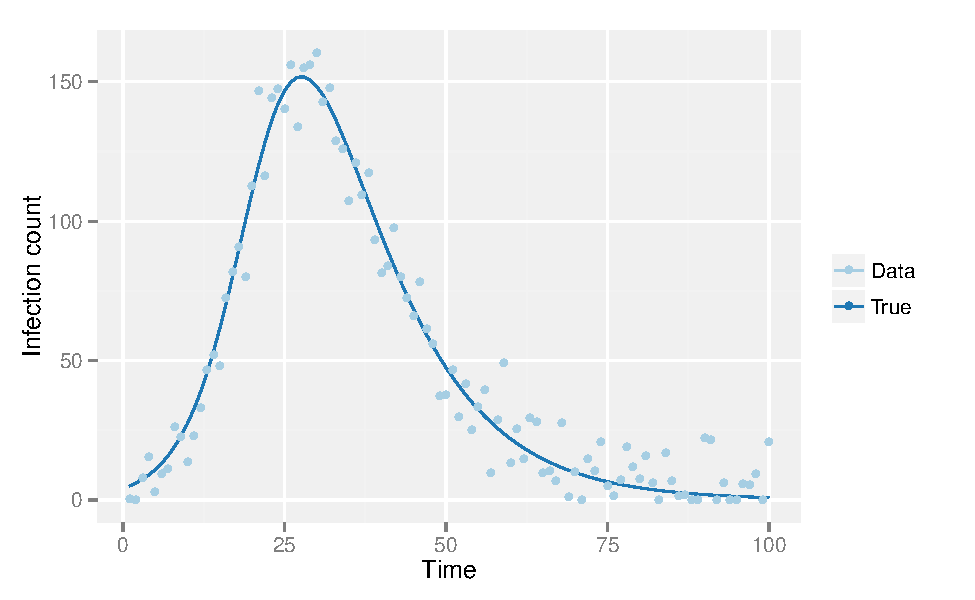
\includegraphics[width=\textwidth]{./images/dataplot.pdf}
        \caption{True SIR ODE solution infected counts, and with added observation noise}
        \label{dataplot}
    \end{figure}
    \fi

\newpage
\begin{appendices}

	\section{Full R code}

    This code will run all the indicated analysis and produce all plots.

    %\lstinputlisting[style=Rsty]{../../Rstan_stuff/sir_stan.r}

    \section{Full C++ code}

    Stan model code to be used with the preceding R code.

    %\lstinputlisting[style=Stansty]{../../Rstan_stuff/sirode_euler.stan}

\end{appendices}







\end{document}